\documentclass[12pt]{article}
\usepackage{kotex,geometry,graphicx,makecell,tabularx,titling,subcaption,booktabs,multirow,amsmath,float}
\usepackage[iso]{datetime}
\usepackage[table]{xcolor}
\usepackage[capitalise]{cleveref}
\usepackage[backend=biber,style=ieee]{biblatex}

\addbibresource{src.bib}
\geometry{a4paper,margin=20mm}
\setlength{\droptitle}{-20mm}
\graphicspath{{./}}
\linespread{1.2}
\pagestyle{empty}
\setlength{\heavyrulewidth}{1.5pt}
% \renewcommand{\arraystretch}{1.5}

\title{IoT 프로젝트 개발 계획서 8조}
\author{
    \vspace{-5mm}
    김준교\thanks{These authors contributed equally.}\protect\phantom{\footnotesize 1}\thanks{School of Electronics and Electrical Engineering, Sungkyunkwan University.} \and
    김찬\footnotemark[1]\protect\phantom{\footnotesize 1}\footnotemark[2] \and 김태형\footnotemark[1]\protect\phantom{\footnotesize 1}\footnotemark[2] \and
    신태하\footnotemark[1]\protect\phantom{\footnotesize 1}\thanks{School of Mechanical Engineering, Sungkyunkwan University.}
    \vspace{-5mm}
}
\date{\today}

\begin{document}
    \maketitle
    \thispagestyle{empty}
    \vspace{-10mm}
    \section{개요}
            \paragraph{{\textbf{제목}}} 팜 덥니?
            \paragraph{\textbf{개발 기간}} 2025-03-13 (Thu.)/06-05 (Thu.)
            \paragraph{\textbf{참여인력 현황 및 담당업무}}
            \begin{itemize}
                \item 신태하(조장): 3D 모델링 및 프린팅, 가속도 측정 및 관련 알고리즘
                \item 김준교: 모바일 앱, 서버 및 통신 프로세스 개발 담당
                \item 김찬: 수로 제어, 하드웨어 담당
                \item 김태형: 수로 제어, 하드웨어 담당
            \end{itemize}
    \section{목표}
        \subsection{개발 목표}
                \paragraph{\textbf{\textcolor{red}{농민들의 온열 질환으로 인한 인명 사고}}}
                \cref{news}와 \cref{ch}는 본 문제의 심각성을 제시합니다.\cite{news}
                질병관리청의 발표자료\cite{src}에 따르면 농업 종사자 중 온열 질환자 수는 \cref{bar}와 같이 2023년 503명에서 2024년 667명으로 증가하였습니다.
                \cref{pie}에서 볼 수 있듯, 이는 전체 온열 질환자 중 약 18\%의 비중을 차지하는 수치로, 심각성이 대두되고 있습니다.
            \begin{figure}[H]
                \centering
                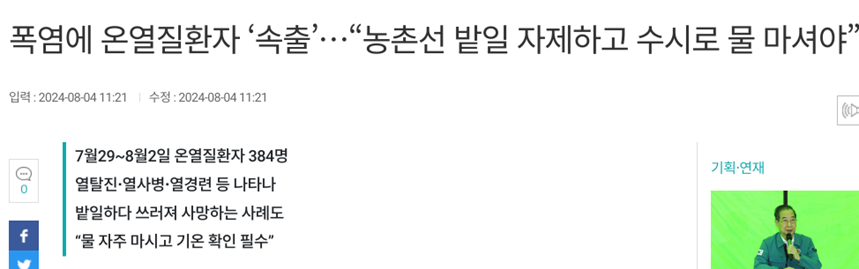
\includegraphics[width=.5\textwidth]{news.png}
                \caption{문제 인식}
                \label{news}
            \end{figure}
            \begin{figure}[h]
                \centering
                \begin{minipage}{.8\textwidth}
                    \centering
                    \begin{subfigure}{.4\textwidth}
                        \centering
                        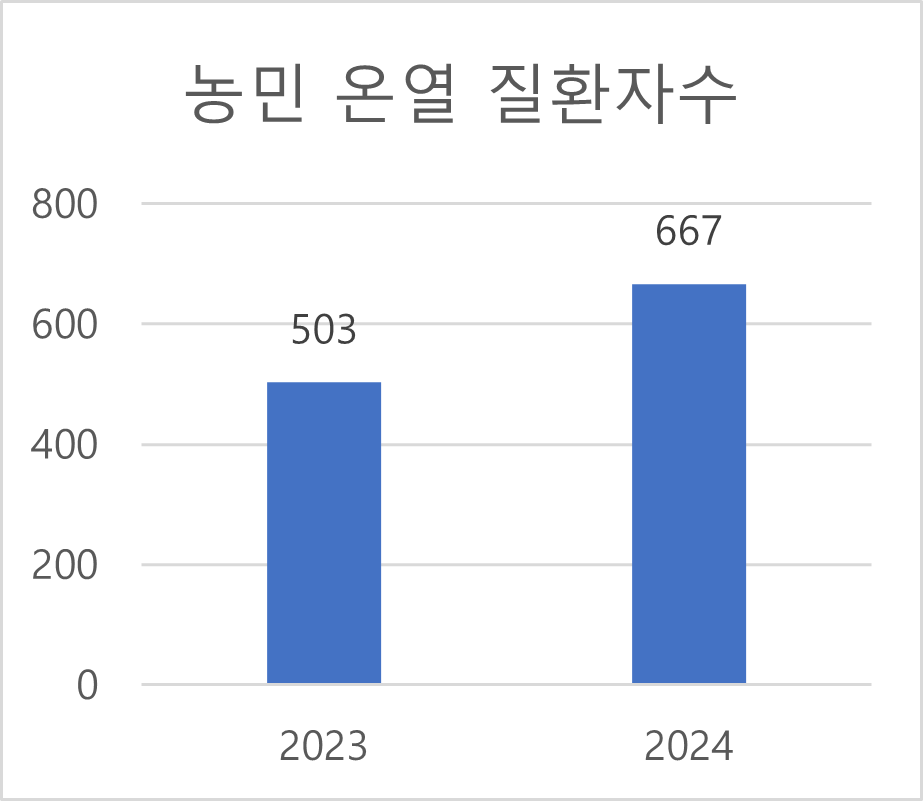
\includegraphics[width=\linewidth]{chart1.png}
                        \caption{질환자 추이}
                        \label{bar}
                    \end{subfigure}
                    \hfill
                    \begin{subfigure}{.4\textwidth}
                        \centering
                        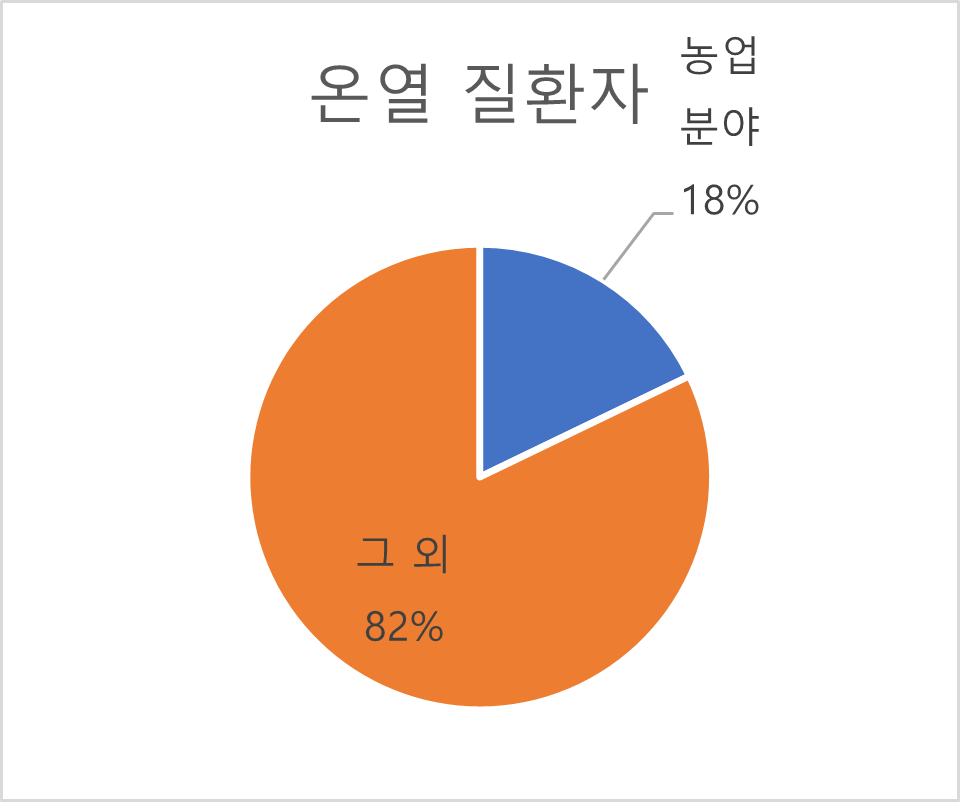
\includegraphics[width=\linewidth]{chart2.png}
                        \caption{질환자 비중}
                        \label{pie}
                    \end{subfigure}
                    \caption{문제 현황}
                    \label{ch}
                \end{minipage}
            \end{figure}

            \paragraph{\textbf{\textcolor{blue}{농민의 체온 이상 해결 시스템}}}
            `팜 덥니?' 시스템은 열사병 등의 온열 질환의 예방에 일차적인 목적을 둡니다.
            추가적으로 긴급 상황 구조 체계를 통해 의식을 잃는 경우에도 대응할 수 있습니다.
            \begin{itemize}
                \item 체온 이상 해결
                \begin{itemize}
                    \item 일정 수준 이상의 체온에 도달했을 때, 위치한 구역의 스프링클러를 작동시킵니다.
                    \item 체온이 다시 정상 범위에 도달하면 스프링클러 작동을 중단시킵니다.
                    \item 많은 농장에서 사용 중인 병렬 관개 시스템과 연계하여 제어됩니다.
                \end{itemize}
                \item 긴급 상황 구조 체계
                \begin{itemize}
                    \item 웨어러블 기기로 단위 시간 별 자세 변화 유무를 쓰러짐 유무를 판단합니다.
                    \item 쓰러졌다고 판단되면, 사용자의 의식을 묻는 작업을 거칩니다. 의식 불명 확인 시, 위치 정보를 포함한 구조 신호가 구조 기관(119 등)에 전송됩니다.
                \end{itemize}
            \end{itemize}
            \paragraph{\textbf{제품 기대효과}}
                이 시스템은 추후 농장을 벗어나 공사 현장, 야외 경기장 등으로 확장 적용될 수 있을 것입니다. 또한 일사병을 예방하기 위한 기능 뿐만 아니라, 다양한 사고로 의식을 잃는 상황에도 대처할 수 있는 종합적인 솔루션을 제공합니다
        \subsection{차별화}
            `팜 덥니?' 시스템은 사용자의 착용 부담을 줄이고, 자동 조작으로 번거로움을 해소하였습니다.
            기존 온열 질환 해결 제품과의 차이점을 \cref{diff}에 정리하였습니다.
        % \newpage
            \begin{table}[H]
                \centering
                \caption{시장조사 및 비교}
                \label{diff}
                \begin{tabular}{c|ccc>{\columncolor{blue!25}}c}
                    \toprule
                    %\rowcolor{blue!25}
                    평가기준 & 선풍기 조끼\cite{fan} & 수냉식 조끼\cite{chill} & 물 분무 선풍기\cite{scatter}& \textbf{팜 덥니?} \\
                    \midrule
                    착용 여부 & O & O &X & $\Delta$\\
                    해결 방식 & 선풍기 & 수냉식 얼음 & 물 분무 & 물 분사 \\
                    작동 기준 & 직접 조작 & 직접 착용 & 직접 조작 & 자동 조작 \\
                    % \midrule
                    % \multicolumn{1}{c}{}&\multicolumn{1}{c}{\includegraphics[width=.1\linewidth,height=.12\linewidth]{fan.png}}&\includegraphics[width=.1\linewidth,height=.12\linewidth]{chill.png}&\includegraphics[width=.1\linewidth,height=.12\linewidth]{scatter.png}&\includegraphics[width=.1\linewidth]{check.png}\\
                    \bottomrule
                \end{tabular}
            \end{table}
    \section{개발 내용}
        \subsection{세부 일정표}
            \cref{Schedule}에 대략적인 주차별 계획을 작성하였습니다. 이는 개발 과정에 따라 변동될 수 있습니다.
            \begin{table}[H]
                \centering
                \caption{Schedule}
                \label{Schedule}
                \begin{tabular}{c|l}
                    \toprule
                    주차&\makecell[c]{내용}\\
                    \midrule
                    4& 계획 구체화, 워크플로우 구상\\
                    5& MPU/MCU 개발보드 연습 및 센서 테스트\\
                    6& 기능 구현 시작: 백엔드/관개수로 모형화/모터 제어/가속도 추출 등\\
                    7-9& 개별 기능 구현 완료(중간 평가)\\
                    10& 개별 기능 보충 및 기능별 연계 시작\\
                    11& 로직 완성\\
                    12-13& 연계 완성\\
                    14& 최종 캘리브레이션, 트러블슈팅\\
                    15& 완성(최종 평가)\\
                    \bottomrule
                \end{tabular}
            \end{table}
        % \newpage
        \subsection{전체 구성도}
            \cref{dia}에 전체 시스템 구성을 도시하였습니다. 세부적인 구현은 변동될 수 있습니다.
            \begin{figure}[H]
                \centering
                % \begin{minipage}{.8\textwidth}
                    % \centering
                    \begin{subfigure}{.6\textwidth}
                        \centering
                        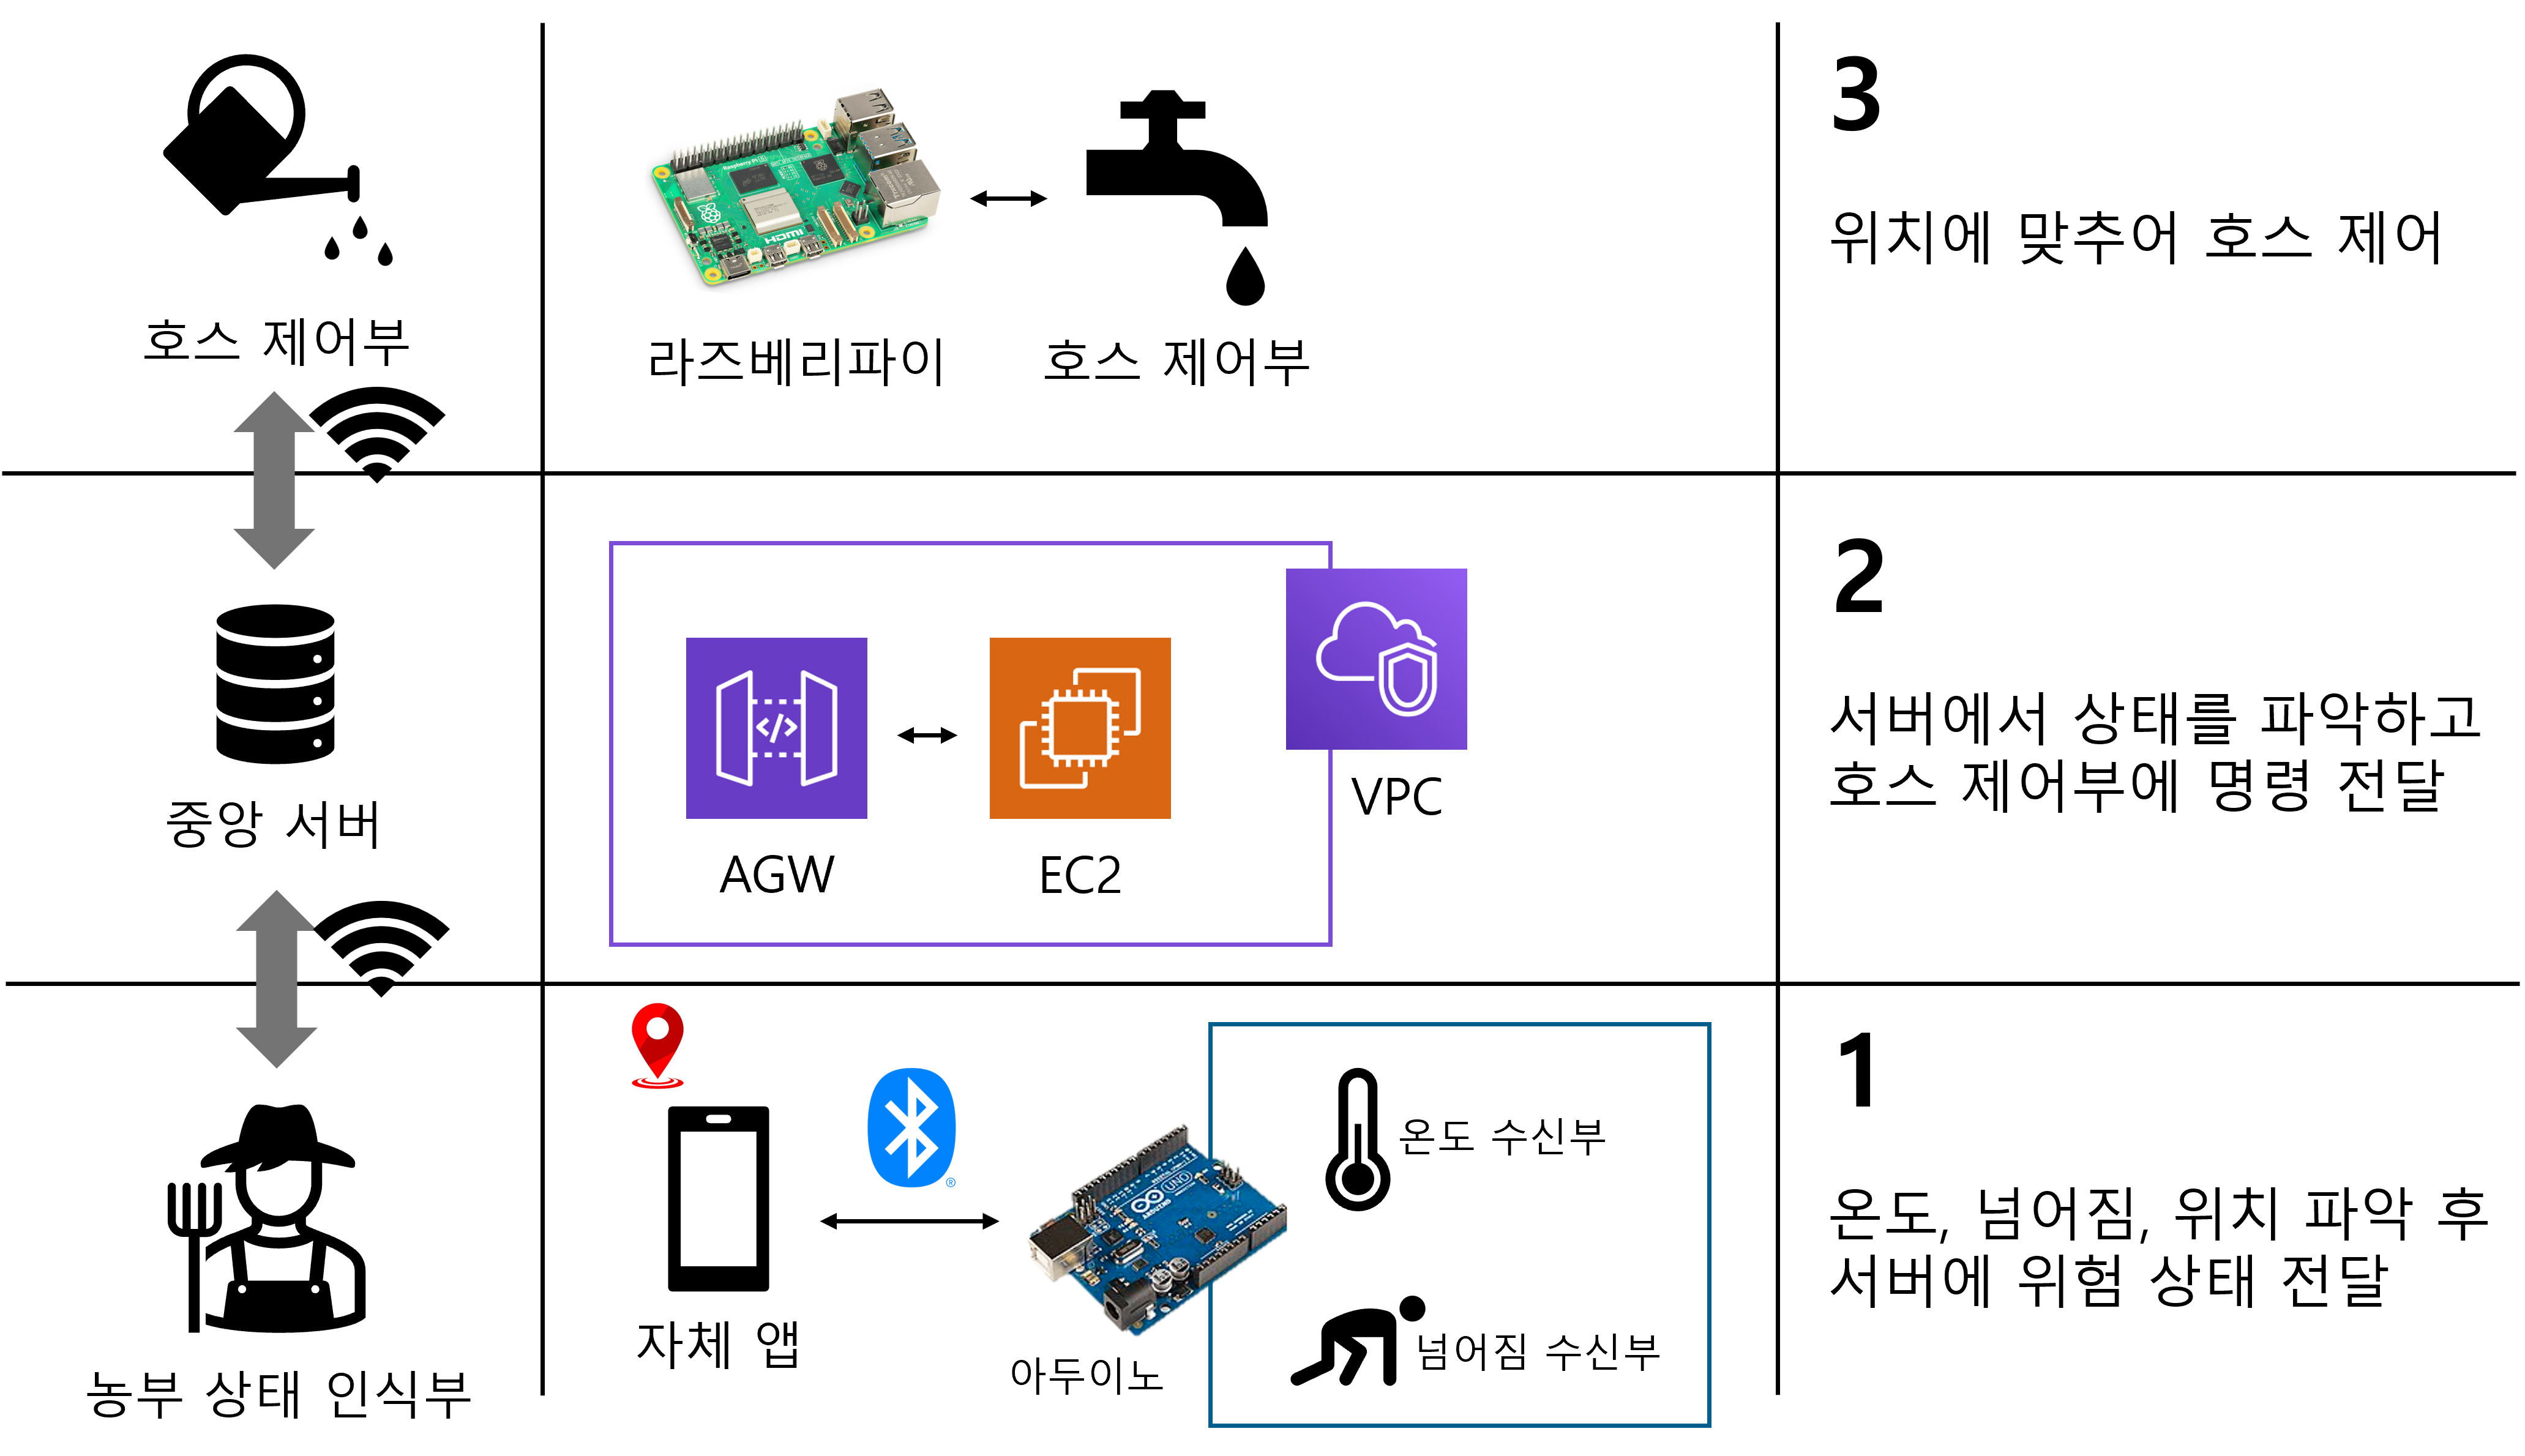
\includegraphics[width=\linewidth]{diagram.png}
                        \caption{시스템 모식도}
                        \label{dia1}
                    \end{subfigure}
                    \hfill
                    \begin{subfigure}{.3\textwidth}
                        \centering
                        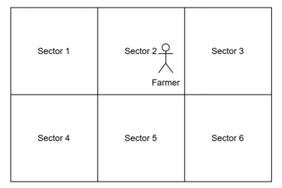
\includegraphics[width=\linewidth]{user.png}
                        \caption{농장의 Sector와 사용자의 위치 예시(GPS)}
                        \label{dia2}
                    \end{subfigure}
                % \end{minipage}
                \caption{전체 구성}
                \label{dia}
            \end{figure}
        \newpage
        \subsection{상세 설명}
            `팜 덥니?' 시스템에는 두 개의 워크플로우가 있습니다.
            \paragraph{체온 이상 시나리오}다음과 같은 순서로 문제를 해결하며, 이를 도식화하여 나타내면 \cref{flow1}의 플로우차트와 같습니다.
            \begin{enumerate}
                \item \textbf{체온 측정}(온도 센서): 사용자의 체온 데이터를 주기적으로 수집하여 I\textsuperscript{2}C 통신으로 아두이노에 전달합니다.
                \item \textbf{체온 이상 여부 확인}(아두이노): 설정된 정상 체온 범위와 비교하여 위험 수준인지 판단하고, Bluetooth 통신으로 모바일 앱에 전달합니다.
                \item \textbf{사용자 상태 갱신}(모바일 앱): 사용자 상태를 주기적으로 갱신하고, 상태 이상 시 서버에 Cellular 통신으로 GPS 위치 정보를 전달합니다.
                \item \textbf{정보 송수신}(중앙 서버): 수신된 위치 정보를 통해 사용자가 농장의 어느 Sector에 있는지 파악하고, API response로 라즈베리파이에 지시를 내립니다.
                \item \textbf{특정 스프링클러 작동}(라즈베리파이): 서버에 주기적으로 갱신을 요청하고, response를 받을 경우 해당 Sector의 스프링클러를 작동시킵니다.
            \end{enumerate}
            \begin{figure}[H]
                \centering
                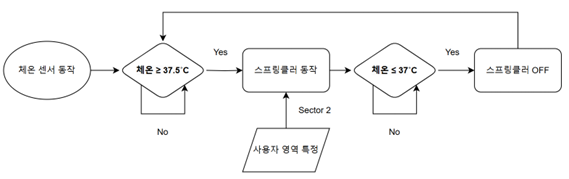
\includegraphics[width=.8\linewidth]{flow1.png}
                \caption{Flowchart of Temperature Anormaly Scenario}
                \label{flow1}
            \end{figure}

            % \begin{table}[H]
            %     \centering
            %     \caption{Operation of Temperature Anormaly Scenario}
            %     \label{table1}
            %     \begin{tabular}{clcl}
            %         \toprule
            %         순서& 목적& 디바이스& 기능\\
            %         \midrule
            %         1& 체온 측정& 온도 센서&\makecell[l]{체온 데이터를 주기적으로 수집,\\아두이노로 전달}\\
            %         \cmidrule(lr){4-4}
            %         2&체온 이상 여부 확인&아두이노&\makecell[l]{설정된 체온 범위로 위험 수준을 판단,\\모바일 앱으로 전달(Bluetooth)}\\
            %         \cmidrule(lr){4-4}
            %         3&사용자 상태 갱신&모바일 앱&\makecell[l]{사용자 상태를 주기적으로 갱신,\\상태 이상 시 서버에 위치 정보 전달\\(GPS, Cellular 활용)}\\
            %         \cmidrule(lr){4-4}
            %         4&정보 송수신&중앙 서버(AWS)&\makecell[l]{위치 정보를 통해 사용자의 Sector 파악,\\ API response로 라즈베리파이에 지시}\\
            %         \cmidrule(lr){4-4}
            %         5&특정 스프링클러 작동& 라즈베리파이&\makecell[l]{사용자의 Sector 정보에 대해\\서버에 주기적으로 갱신 요청}\\
            %         \bottomrule
            %     \end{tabular}
            % \end{table}
            % \newpage
            \paragraph{긴급 상황 시나리오}다음과 같은 순서로 문제를 해결하며, 이를 도식화하여 나타내면 \cref{flow2}의 플로우차트와 같습니다.
            \begin{enumerate}
                \item \textbf{심박수 및 움직임 측정}(심박 센서, 가속도 센서): 사용자의 심박수 및 신체 가속도 데이터를 주기적으로 수집하여 I\textsuperscript{2}C 통신으로 아두이노에 전달합니다.
                \item \textbf{이상 여부 확인}(아두이노): 심박수 및 움직임 데이터를 설정된 기준값과 비교하여 사용자의 의식 여부를 판단하고 Bluetooth 통신으로 모바일 앱에 전달합니다.
                \item \textbf{사용자 상태 확인}(모바일 앱): 상태 이상 신호를 수신할 경우, 진위 판정을 위해 사용자의 응답을 요구합니다.
                \item \textbf{응급 신호 전송}(모바일 앱): 특정 시간 동안 사용자가 응답하지 않는다면 구조 기관에 응급 신호를 전송합니다.
            \end{enumerate}
            \begin{figure}
                \centering
                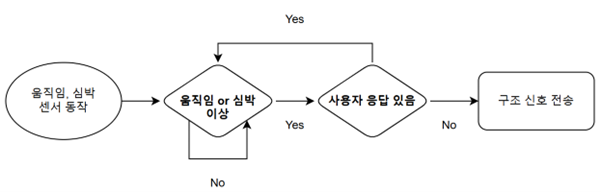
\includegraphics[width=.8\linewidth]{flow2.png}
                \caption{Flowchart of Emergency Scenario}
                \label{flow2}
            \end{figure}

            % \begin{table}[H]
            %     \centering
            %     \caption{Operation of Emergency Scenario}
            %     \label{table2}
            %     \begin{tabular}{clcl}
            %         \toprule
            %         순서&	목적&	디바이스&	기능\\
            %         \midrule
            %         1&심박수 및 미동 확인&심박 센서, 가속도 센서&\makecell[l]{사용자 의식 확인을 위한\\데이터를 아두이노로 전달}\\
            %         \cmidrule(lr){4-4}
            %         2&이상 여부 확인&아두이노&\makecell[l]{움직임 또는 심박의 변화로\\사용자 의식 여부를 판단,\\모바일 앱으로 전달}\\
            %         \cmidrule(lr){4-4}
            %         3&사용자 상태 확인&모바일 앱&\makecell[l]{상태 이상 신호 수신,\\진위 여부 판단을 위해\\사용자의 응답을 요구}\\
            %         \cmidrule(lr){4-4}
            %         4&구조 신호 전송&모바일 앱&\makecell[l]{사용자의 무응답,\\이에 따른 구조 신호 전송}\\
            %         \bottomrule
            %     \end{tabular}
            % \end{table}
    \printbibliography
\end{document}